\section{Visual Simulation of Smoke 解説}
Visual Simulation of Smoke\cite{Fedkiw2001}を解説する。
物理シミュレーションの実装に必要なアルゴリズムを中心に説明する。
\subsection{概要}
煙のようなガスをシミュレートするためのモデルを提案する。
煙の速度を非圧縮性のオイラーの運動方程式でモデル化する。
非圧縮性のオイラーの運動方程式はセミラグランジュ法と圧力のポアソン方程式を用いて解く。
数値拡散を減らす渦度強制(Vorticity Confinment)の手法を提供する。
このモデルは安定的、高速かつ数値拡散を起こすことがない。
\subsection{方程式}
気体のモデルとして非粘性、非圧縮、粘度が一定の気体を仮定する。
粘性、圧縮性は気体のシミュレーションでは無視できる。
煙の速度 $\upsilon = (u,v,w)$は非圧縮のオイラーの運動方程式によって与えられる。
\begin{equation}
\label{continuity}
\nabla \cdot \upsilon = 0
\end{equation}
\begin{equation}
\label{euler}
\frac{\partial \upsilon}{\partial t} = -(\upsilon \cdot \nabla)\upsilon - \nabla p + f
\end{equation}
式(\ref{continuity})は質量保存、式(\ref{euler})は運動量保存を表す。
$p$は気体の圧力、$f$は外力を表す。
式(\ref{euler})の右辺は左から移流項、圧縮項、外力項と呼ぶ。

これらの式を2段階で解く。
はじめに式(\ref{euler})の左辺で時間刻み幅$\Delta t$を利用し、
右辺の圧縮項をなくした式(\ref{advection})を解いて中間速度場$u^*$を求める。
\begin{equation}
\label{advection}
\frac{\upsilon^* - \upsilon}{\Delta t} = -(\upsilon \cdot \nabla)\upsilon + f
\end{equation}
次に中間速度場$u^*$をプロジェクション法によって非圧縮性を満たすようにする。
これはノイマン境界条件にしたがった以下のポアソン方程式から圧力を計算することに等しい。
\begin{equation}
\label{poisson}
\nabla^2 p = \frac{1}{\Delta t} \nabla \cdot \upsilon^*
\end{equation}
式(\ref{poisson})の導出をする。まず最終的な速度場を$\upsilon$とした場合に$\frac{\upsilon - \upsilon^* }{\Delta t} = - \nabla p$となる。これに両辺の発散をとる($\nabla$を掛ける)と$\frac{\nabla \cdot \upsilon - \nabla \cdot \upsilon^*}{\nabla t} = - \nabla^2 p$ となる。式(\ref{continuity})$\nabla \cdot \upsilon = 0$から$- \frac{\nabla \cdot \upsilon^*}{\nabla t} = - \nabla^2 p$となりこれを式変形することで式(\ref{poisson})が導出できる。

中間速度場から圧力の勾配を引くと非圧縮性を満たす速度となる。
\begin{equation}
\label{getIncompressibleVelocity}
\upsilon = \upsilon^* - \Delta t \nabla p
\end{equation}
式(\ref{getIncompressibleVelocity})は$\frac{\upsilon - \upsilon^* }{\Delta t} = - \nabla p$の両辺に$\Delta t$を掛けて式変形することで導出できる。

気温$T$と煙の密度$\rho$は煙の速度に沿って運ばれることを仮定する。
\begin{equation}
\label{temperature}
\frac{\partial T}{\partial t} = - ( \upsilon \cdot \nabla)T
\end{equation}
\begin{equation}
\label{temperature}
\frac{\partial \rho}{\partial t} = - ( \upsilon \cdot \nabla)\rho
\end{equation}

濃い煙は重力によって下に落ち、熱い気体は浮力によって上に上がる。
\begin{equation}
\label{buoyancy}
f_{buoy}=-\alpha\rho z + \beta(T-T_{amb}) z
\end{equation} 
$z=(0,0,1)$は上の垂直方向のベクトル、$T_{amb}$は大気の環境温度、
$\alpha$と$\beta$は正の定数となる。

数値拡散によって細かい渦の挙動が失われる。
渦度強制により検出した渦の情報を元に速度場に速度を追加することで渦の消失を防ぐ。
最初に渦$\omega$を取得する。
\begin{equation}
\label{volticity}
\omega=\nabla \times \upsilon
\end{equation}
低い渦濃度から高い渦濃度へのベクトルを正規化する。
\begin{equation}
\label{normalizeVelocityLocation}
N=\frac{\eta}{|\eta|}\;(\eta=\nabla|\omega|)
\end{equation}
以下より追加する外力を求める。
\begin{equation}
\label{confinementForce}
f_{conf}=\epsilon h (N \times \omega)
\end{equation}
$\epsilon > 0$は追加する渦のスケール、$h$は格子幅を表す。
\subsection{実装}

空間の差分化は同一の大きさの格子に分割する格子法(図\ref{grid})を用いる。
格子の中心には煙の密度、温度、外力が定義されるのに対して、格子の面には速度が定義される。
この格子をスタガード格子と呼ぶ。
スタガード格子は通常の格子と比べて人工的な散逸を減らす。

\begin{figure}
	\begin{center}
		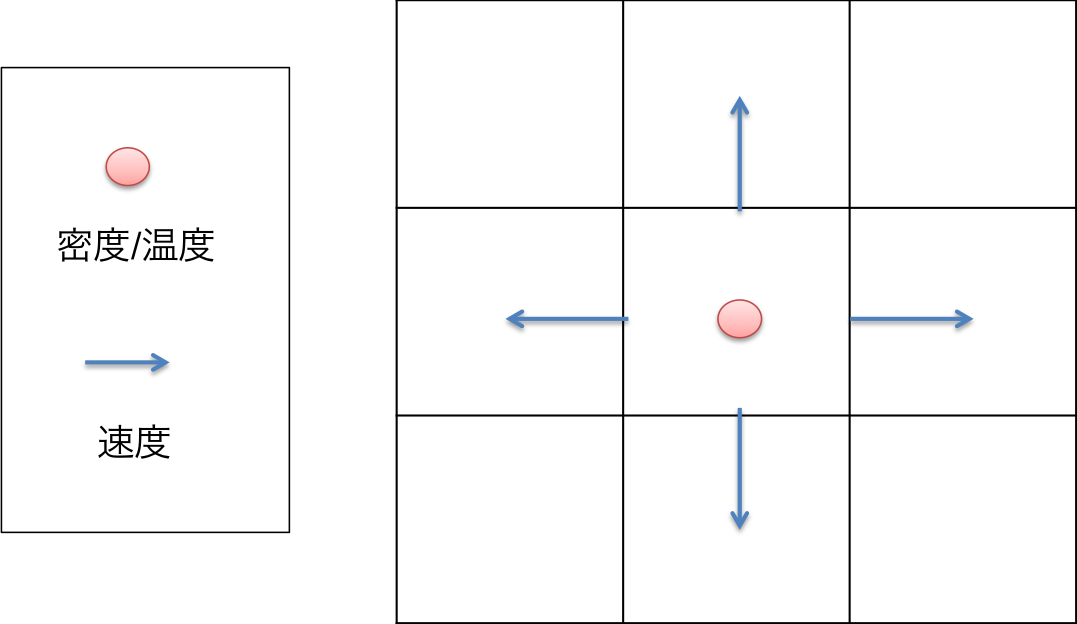
\includegraphics[width=100mm]{grid.png}
		\caption{空間の差分化}
		\label{grid}
	\end{center}
\end{figure}


処理全体の流れ(図\ref{overview})は流体の速度の計算を行い、計算した速度から煙の密度の計算を行うことを繰り返す。
流体の速度はオイラーの運動方程式(\ref{euler})を外力項、移流項、圧縮項の計算結果を足すことにより計算する。

\begin{figure}
	\begin{center}
		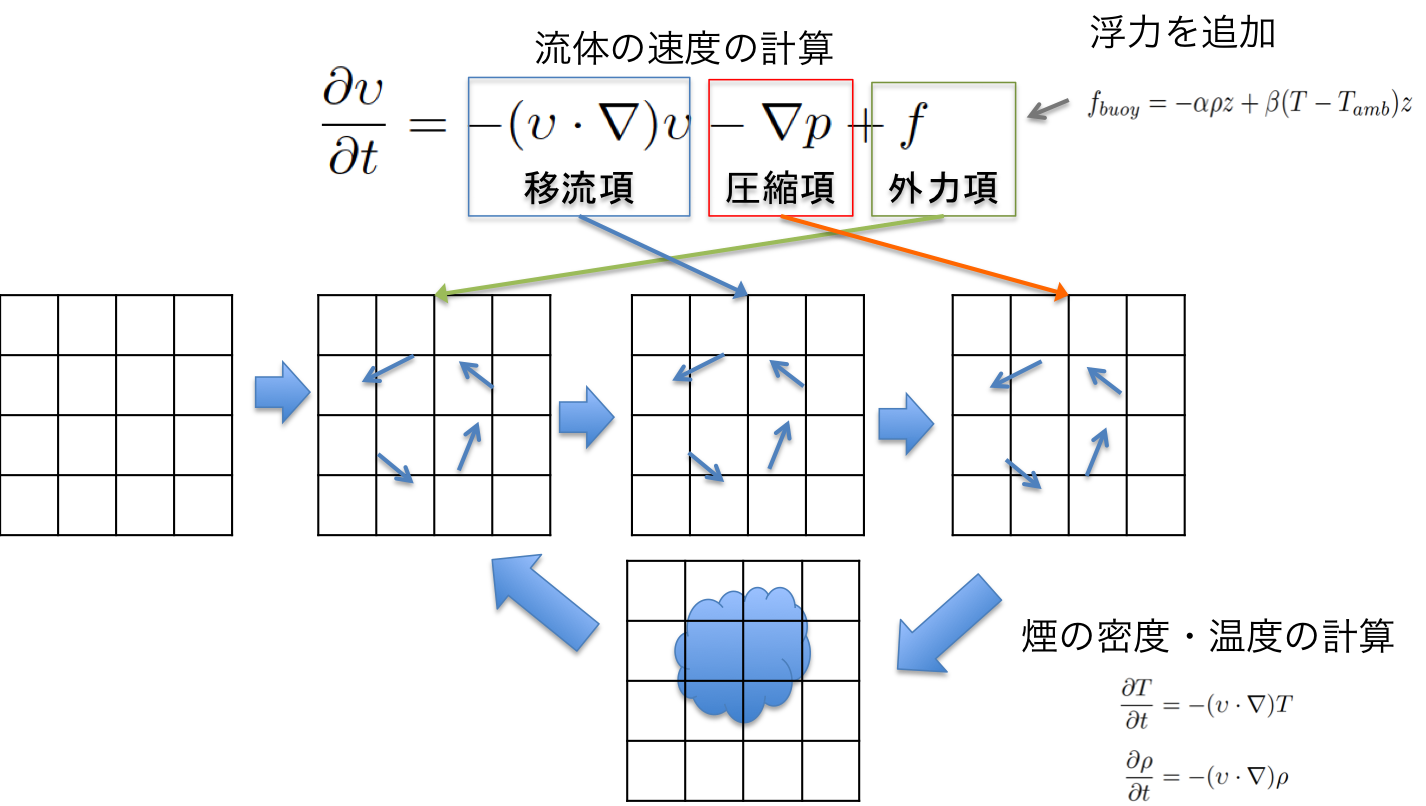
\includegraphics[width=100mm]{overview.png}
		\caption{処理全体の流れ}
		\label{overview}
	\end{center}
\end{figure}

すべての物理量を格納する格子を2つ用意する。
時間刻み幅$\Delta t$により修正された格子を、もう一つの格子に更新する。

はじめに外力から速度を更新する。
外力にはユーザからの与えられる力、式(\ref{buoyancy})に定義される浮力、
式(\ref{confinementForce})に定義される渦度強制による力がある。

次に式(\ref{advection})の移流項をセミラグランジュ法によって解く。
セミラグランジュ法とは速度場をバックトレースすることで求める方法である。新しい速度はバックトレースした点にある速度場から補完する。
バックトレースした点が格子の外の場合がある。
この場合、単純にバックトレースする経路を境界面で切り取る。

補間にエルミート補間を利用した場合、オーバーシュートが起こる。
提案するキュービック補間は単調でオーバーシュートしない。

最後に速度場を質量保存則に従うようにする。
圧力を求めるためポアソン方程式(\ref{poisson})を解く。
この方程式の差分化の結果は疎な連立一次方程式になる。
法線方向の圧力勾配が0のノイマン境界条件を使う。
連立方程式は共役勾配法(CG法)が実装が容易で収束性質が良い。
収束を良くするため不完全コレスキー分解を用いる。
これは標準的な方法である。
圧力を求めた後、速度から圧力の勾配を引く。

速度が更新されたら、セミラグランジュ法を再び用いて気温と煙の密度を移流する。

